% ##################################################################################################################
\chapter{MATSim Data Containers}
\label{sec:extending-data-containers}
%% \subsection{Supply-Side Data Containers}
%% \label{sec:supplysidemodules}
%% % ======================================================
%% \subsection{Scenario}
%% \label{sec:extending-scenario}

%% The \lstinline|scenario| module is
%% %, on the one hand, 
%% a container containing the main components of a scenario such as the \lstinline|config|, the \lstinline|network|, the \lstinline|population|, the \lstinline|facilities|, 
%% %the \lstinline|transitSchedule| \kai{unclear}, 
%% \lstinline|households| and \lstinline|vehicles|.

%% From a configuration perspective, the containers are available when a filename is given, otherwise not.  If an invalid filename is given, the code aborts with an error message.  If the code is configured in a way that it needs a container that was not loaded, it also aborts with an error message.

%% There are also switches of type 
%% \begin{xml}
%% <param name="useHouseholds" value="..."/>
%% \end{xml} in the \lstinline|scenario| module of the \gls{configfile}.  
%% These are deprecated and will eventually go away.  
%% Until then, it may be that they have to be set correctly for the code to function. \atend{chk if useXxx switches in scenario have gone}

%% From a programming perspective, arbitrary additional containers can be plugged into the global \lstinline|scenario| container.  
%% See Section \ref{sec:scenario-extension-point} for more details.

%% \begin{itemize}\styleItemize
%% \item Invoking the module: (1) if you use Controler, scenario is always there. (2) otherwise, it needs to be generated explicitly in java.  \kai{chk}
%% \kai{Wir sind uns nicht im klaren darüber, was diese switches genau bedeuten, siehe \url{https://matsim.atlassian.net/browse/MATSIM-320}.  $\to$ weglassen.}

%% \item Configuration: There is a \lstinline|scenario| config file section, but we don't know what it means. \kai{chk} \ah{Hier haben wir doch eine kleine Inkonsistenz zwischen Container und Configuration Section. Config section definiert lanes, signals, households, vehicles, transit. Scenario hat aber z.B. facilities und population drin. Man sollte diese config section evtl. umbenennen in sowas wie optional\_scenario\_elements oder ähnlich. \url{https://matsim.atlassian.net/browse/MATSIM-320}}
%% \end{itemize}

%% The config file section is, on the other hand, used in a slightly different manner. It defines the usage of lanes, signal systems, road pricing, agent knowledges, vehicles, households and public transport. Still a respective config file section is required for every additional functionality. \kai{Ist das genau so?  Ich habe da ehrlich gesagt das genaue Design nie verstanden.  Oft für ein Eintrag in der scenario config group nur dafür, dass die Daten gelesen werden, und sonst passiert gar nichts.  Hm ...  Geradeziehen???}

% Code: \lstinline|org.matsim.core.scenario|

% ===================================================================================
\subsection{Time-dependent Network}
\label{sec:extending-network}

The network container was already described in Section~\ref{sec:using-network}.
%
An important additional feature of the network module is using time-dependent network attributes. Network state changes can thus be considered, as \eg implied by accidents, or adaptive traffic control, with varying speed limits or driving directions of lanes on multi-lane roads with heavily unbalanced loads over the course of a day. Attributes that can be adapted are ``free speed'', ``number of lanes'' and ``flow capacity''.

The adaptation can be specified by adding the following two lines to the \lstinline|network| \gls{configfile} section:
\begin{xml}
<param name="timeVariantNetwork" value="true" />
<param name="inputChangeEventsFile" value="path_to_change_events_file" />
\end{xml}
%
An example snippet setting the free speed of three network links to zero looks something like this:
%
%% <?xml version="1.0" encoding="UTF-8"?>
%% 	<networkChangeEvents xmlns="http://www.matsim.org/files/dtd"
%% 	xmlns:xsi="http://www.w3.org/2001/XMLSchema-instance"
%% 	xsi:schemaLocation="http://www.matsim.org/files/dtd
%% 	http://www.matsim.org/files/dtd/networkChangeEvents.xsd">}
\begin{xml}
<networkChangeEvent startTime="03:06:00">
   <link refId="12487"/>
   <link refId="12489"/>
   <link refId="12491"/>
   <freespeed type="absolute" value="0.0"/>
</networkChangeEvent>
\end{xml}
%% </networkChangeEvents>
%
%\kai{add reference to real file}
%\ah{no suitable one found :(}
%\kai{Wir sollten eines nach examples/equil-extended einstellen.}
%\ah{done}
For a working example, see the file \lstinline|networkChangeEvents.xml| in the \lstinline|examples/equil-extended| directory in the \gls{matsim} directory tree.

Alternatively, network change events can be added directly to the code.
 %% using the method \lstinline|createNetworkChangeEvent| in class \lstinline|NetworkFactoryImpl|. An example can be found under 
 %% \lstinline|org.matsim.integration.timevariantnetworks.QSimIntegrationTest| class.
An example can be found in the \lstinline{RunTimeDependentNetworkExample} class under \url{http://matsim.org/javadoc} $\to$ main distribution.

Note that change values of type absolute need to be given in \glsunset{si}\gls{si} units, which means speeds in meters per second and flow capacities in vehicles per second.

%% \kaitodo{Write RunXxx example!}
%% \ahtodo{Write RunXxx example!}

 %\ah{unfortunately no javadoc}
%
%\begin{lstlisting}
%networkChangeEvent =
	%network.getFactory().createNetworkChangeEvent(...);
%networkChangeEvent.setFlowCapacityChange(new ChangeValue(...));
%networkChangeEvent.setFreespeedChange(new ChangeValue(...));
%networkChangeEvent0.setLanesChange(new ChangeValue(...));
%network.addNetworkChangeEvent(networkChangeEvent);
%\end{lstlisting}
%
%\kai{lieber ein Verweis auf ein code snippet?  U.a. muss man auf NetworkImpl casten, was wir gerne irgendwann loswerden wollen und daher nicht im Buch haben wollen.}

% Code: \lstinline|org.matsim.core.network|

% ===================================================================================
\subsection{Person Attributes and Subpopulations}
\label{sec:extending-population}

The population container was also already discussed earlier, in Section~\ref{sec:using-population}.
%
A powerful extension of a standard population can be achieved by specifying further agent attributes in an \lstinline|ObjectAttributes| file input to \gls{matsim} by the parameter \lstinline|inputPersonAttributesFile|. 
%% Furthermore, subpopulations can be defined by parameter \lstinline|subpopulation|.
%
% not sure what this means. Maybe it is meant in relation to strategies but this would have to be stated more precisely IMO. kai, jul'15

See \javadoc\ $\to$ main distribution $\to$ \lstinline{RunSubpopulationsExample} class for an example.  That example looks as if coding in \gls{java} is necessary, but this is really not the case; \gls{java} is just used to generate the subpopulations, which could also  be done by other means.

% Code: \lstinline|org.matsim.core.population|

% ===================================================================================
\subsection{Counts}
\label{sec:extending-counts}
By providing a counts input file and configuring the \lstinline|counts| \gls{configfile} section, \gls{matsim} plots link volume comparisons between hourly simulated and counted values for motorized individual traffic \citep{Horni_unpub_IVT_2007}. 

Simulating sample populations requires scaling simulated volumes by the \lstinline|countsScaleFactor| parameter, \eg for a 10\,\% population this parameter needs to be set to~10.

\paragraph{Input}
The following listing shows an example of a \lstinline|counts.xml| input file required for traffic count comparisons. 

\begin{xml}
<?xml version="1.0" encoding="UTF-8"?> 
<counts name="example" desc="example counting stations" year="2015"> 
   <count loc_id="2" cs_id="005"> 
      <volume h="1" val="10.0"></volume> 
      <volume h="2" val="1.0"></volume> 
      <volume h="3" val="2.0"></volume> 
      <volume h="4" val="3.0"></volume> 
      <volume h="5" val="4.0"></volume> 
      <volume h="6" val="5.0"></volume> 
      <volume h="7" val="6.0"></volume> 
      <volume h="8" val="7.0"></volume> 
      <volume h="9" val="8.0"></volume> 
      <volume h="10" val="9.0"></volume> 
      <volume h="11" val="10.0"></volume> 
      <volume h="12" val="11.0"></volume> 
      <volume h="13" val="12.0"></volume> 
      <volume h="14" val="13.0"></volume> 
      <volume h="15" val="14.0"></volume> 
      <volume h="16" val="15.0"></volume> 
      <volume h="17" val="16.0"></volume> 
      <volume h="18" val="17.0"></volume> 
      <volume h="19" val="18.0"></volume> 
      <volume h="20" val="19.0"></volume> 
      <volume h="21" val="20.0"></volume> 
      <volume h="22" val="21.0"></volume> 
      <volume h="23" val="22.0"></volume> 
      <volume h="24" val="23.0"></volume> 
   </count> 
</counts>
\end{xml}
For a working example, check the \lstinline{examples/equil} directory in the \gls{matsim} directory tree (\cf Section~\ref{sec:settingUpMatsim}).  

It starts with a header containing general descriptive information about the counts, including a year to describe how current the data is. Next, for each link having real world counts data, hourly volumes can be specified. The network-link is referenced by the \lstinline|loc_id| attribute; in the example, it is link~2. The attribute \lstinline|cs_id| (counting station identifier) can be used to store an arbitrary description of the counting station. Most often, it is used to note the original real world 
%"\Karen { I think you did mean 'world' there, right?}" 
counting station to simplify future data comparison. The hourly volumes, specified by the hour of the day and its value, are optional: That is, a value does not have to be given for every hour. If, for a counting station, data is only available for certain hours of the day (\eg only during peak hours), it is possible to omit the other hours from the \gls{xml} listing. Note that the first hour of the day, from 0:00\,am to 1:00\,am, is numbered as ``1'', and \emph{not} by ``0'' as is often the case in computer science.

\paragraph{Output}
The counts module prints overview summaries for the whole network, but also analyzes for individual links. Also, a google maps-based visualization is available, showing each station with a its load curve (see the example in Figure~\ref{fig:countcomparison}) in a pop-up window.

% ----------
\createfigure%
{Example for a link volumes comparison between simulation and road count values}%
{Example for a link volumes comparison between simulation and road count values}%
{\label{fig:countcomparison}}%
{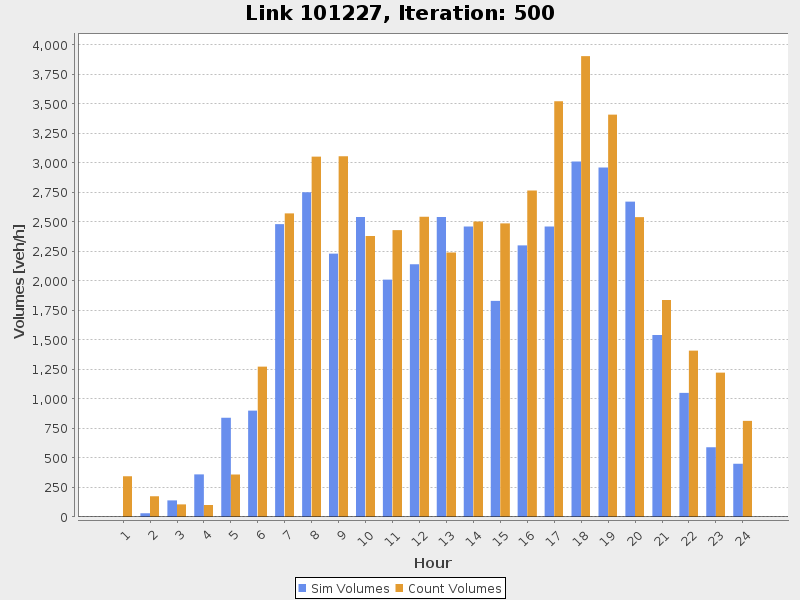
\includegraphics[width=0.7\textwidth, angle=0]{extending/figures/link101227.png}}%
{}
% ----------

%Public transport passenger counts are described in Chapter~\ref{ch:pt}. \ah{check} \ah{nothing there}

\citet[][]{BalmerEtAl_ResRep_bdktzrh_2009} have performed link volume comparisons for the Zürich scenario, with data based on city level, cantonal level and national level \citep[][]{ASTRA_Webpage_2006}.
%% , where an average working day (Monday to Thursday, excluding public holidays) was built. 
Usually, it is helpful to exclude a substantial part of the outer range of the 
modeled study region in order to remove boundary effects.

% Code: \lstinline|org.matsim.counts|

% ===================================================================================
\subsection{Facilities}
\label{sec:extending-facilities}
Facilities are an optional element of \gls{matsim}; some \glspl{module}, such as the destination innovation module (Chapter~\ref{ch:destinationchoice}), depend on it.
If \gls{matsim} \glspl{facility} are used, agents perform their activities in a specific \gls{facility} attached to a network link. 

Facilities are included in the scenario by defining the \lstinline|facilities| \gls{configfile} section and providing a facilities file, approximately as follows.
%
\begin{xml}
...
<facilities name="test facilities for triangle network">
   <facility id="1" x="60.0" y="110.0">
      <activity type="home" />
   </facility>
   <facility id="10" x="110.0" y="270.0">
      <activity type="education" />
   </facility>
</facilities>
\end{xml}
%
In addition to activities that can be done in the facility, further location attributes, such as opening times, can be specified. 
A working facilities example file can be found in the \gls{matsim} directory tree in the \lstinline{examples/siouxfalls-2014} directory.

Facilities are mostly used by the \gls{matsim} Zürich group, in particular in the Zürich scenario, where they are derived from the Federal Enterprise Census~2001 \citep[][]{SwissEnterpriseCensus_manual_2001} providing hectare level information.
%% and using the so-called NOGA-classification. 
% (if the reference to NOGA should remain in the text, the acronym would have to be resolved. kai, dec'15)
Detailed technical description of  facilities generation is given by \citet[][]{Meister_TechRep_IVT_2008}. %Meister_unpub_IVT_2007}. 
%
%\kai{``Meister internal presentation'' keine sinnvolle Referenz?}
Comparable data is available in most countries from official sources, such as censuses, and commercial sources, such as navigation network providers, yellow pages publishers or business directories, and last but not least google and \gls{osm} \citep[][]{OpenStreetMap_Webpage_2015}.

Note that loading a facilities file into \gls{matsim} by itself does not mean they will be used; the functionality needs to be switched on by other means.  Currently, this is only possible by using some class with a \lstinline{main} method.
 %% that can do that.

% Code:\lstinline|org.matsim.core.facilities|

% ##################################################################################################################
%% \subsection{Demand-Side Data Containers}
%% \label{sec:dsm}

% ===================================================================================
\subsection{Households}
\label{sec:extending-households}
Households are another optional element of \gls{matsim}. To load households into a scenario, the %% \lstinline|useHouseholds| parameter in the \lstinline|scenario| \gls{configfile} section must be set to true. Furthermore, the 
\gls{configfile} must 
contain a section \lstinline|households|. This section should specify the paths to a file containing households (parameter \lstinline|inputFile|) and a file containing further household attributes (parameter \lstinline|inputHouseholdAttributesFile|).\footnote{%
%
There used to be an additional ``useHouseholds'' config switch.  In release 0.8.x, that switch will be gone.
%
}

Again, loading the households file does not mean that it is used anywhere in the code; such functionality needs to be switched on separately.  Currently, no such functionality can be switched on from the \gls{configfile} alone.

% \ah{households file listing?} \ah{maybe next revision}

% Code: \lstinline|org.matsim.households|

% ===================================================================================
%% \subsection{Data containers belonging both to demand and to supply}
\subsection{Vehicles}
\label{sec:extending-vehicles}

Vehicles are an optional element of \gls{matsim}. To load vehicles into a scenario, a config section
\begin{xml}
<module name="vehicles" >
   <param name="vehiclesFile" value="/path/to/vehicles.xml.gz" />
</module>
\end{xml}
needs to be added.\footnote{%
%
There used to be an additional ``useVehicles'' config switch.  In release 0.8.x, that switch will be gone.
%
}
%% the \lstinline|useVehicles|\kaitodo{chk the useXxx switches} parameter in the \lstinline|scenario| \gls{configfile} section must be set to true. Furthermore the \gls{configfile} must contain a section \lstinline|vehicles|. This section should specify the paths to a file containing vehicles (parameter \lstinline|vehiclesFile|). 

Once more, just loading the vehicles does not use them; that needs to be configured separately.  See Section \ref{sec:vehicles-in-qsim} for details.


%\citet[][]{JaeggiEtAl_TRR_2012} might serve as an empirical base for the assignment of vehicles to agents or households. \ah{Füllsatz}

%\kai{Andreas, habe jetzt die transitXxx file formats in das pt chapter verschoben.  Meine Intuition ist zwar eigentlich, dass sie besser ``Infrastruktur'' (als ``shared'') Container wären.  Aber Marcel hat das bis jetzt anders gesagt, und es ist auch kein so großes Problem.} \kai{Siehe auch \url{https://matsim.atlassian.net/browse/MATSIM-332}.} \ah{ok}

%\kai{Folgendes muss noch geschrieben werden.} \ah{done}

%% \kai{Bin mir ziemlich sicher, dass wir hier nur die ``vehicles'' lassen sollten, und die ``transitVehicles'' erst mit der entsprechenden extension erklären sollten.  Auch die freightVehicles sind schließlich nicht global verfügbar, sondern nur im Rahmen der extension.}

%% \kai{Folgendes ist nicht operational.  Sehe im Moment gar nicht, wie wir das Buch sinnvoll fertig schreiben können, ohne das gelöst zu haben, aber ich sehe auch nicht, wo die Zeit herkommen soll.}
%% %
%% \kai{Ok, in einem Anfall von Verzweiflung habe ich das gestern eingebaut: vehicles und transitVehicles sind nun separat.  Allerdings laufen die automatischen Tests im Moment irgendwie nicht; das sollte man vielleicht noch abwarten.}

%% \kai{Von der Logik her sollen die ``useXxx'' switches im scenario module der config auch noch weg.  Aber im Moment geht das nicht ohne größeren Umstand.}

%% A private household's decision to buy a vehicle in order to satisfy one's transport needs is a demand side decision.
%% %
%% However, if a public transit company decides to buy buses of a certain type, this is more a supply side decision (to supply potential passengers with a vehicle) than a demand side decision (the vehicle will have a demand for road space once it runs).

%% \begin{itemize}\styleItemize
%% \item Invoking the module: Vehicles need to be enabled in the \lstinline|scenario| configuration file section.
%% \item Configuration: At the moment vehicles are only used for public transport (Chapter~\ref{ch:pt}), \ie motorized individual traffic vehicles are not used in \gls{matsim} nowadays. Thus, the configuration file section specifying the input file is located in the \lstinline|transit| configuration file section, while the vehicles module does not have its own configuration file section. 
%% \ah{Klären, ob man diese kleine Inkonsistenz beheben möchte.}  
%% \kai{Ist das nicht schon erledigt?}
%% \ah{final String vehiclesFile = this.config.transit().getVehiclesFile();}
%% \kai{Arghh.}
%% \ah{\url{https://matsim.atlassian.net/browse/MATSIM-314}}
%% %
%% This might change one day when the parking module will start to use vehicles. 
%% \end{itemize}

%% The vehicles package provides a file reader and a factory to create vehicles.

% Code: \lstinline|org.matsim.vehicles|

\subsection{Scenario}
\label{sec:extending-scenario}

\lstinline{Scenario} is a super-container containing all the other data containers, accessible, for example, as \lstinline{scenario.getNetwork()}.  It used to have configuration options, but these are all gone now, so \lstinline{Scenario} is only visible once you are programming in \gls{java}. 

